\scanpage{62}
\diagram{\resizebox{\linewidth}{!}{$\begin{array}{r|l|l|l|l|l}
 &\substack{\text{Cat :}\\\Delta\text{ munis de}}&\text{équivalente à}&\text{groupe d'autom}&\substack{\text{Cardinal de l'ens des}\\\text{él. de structure}\\\text{du type envis. de }\Delta}&\\ \hline
1^\circ & \substack{\text{1-base}\\ \bullet \qquad /\!/\!/} & \substack{\deleted{\unsure{\text{structure de}}}\ \deleted{\unsure{\text{torseur}}}\\\text{ens }J\text{ de card}\\5,\ \text{et torseur}\\\text{sous }\mathbb F_2(J)'} & \substack{W_{\mathrm{SO}(10)}\quad\text{ext.}\\\text{de }\unsure{\mathfrak S|\mathscr S}_5\text{ par }(\mathbb Z/2\mathbb Z)^4\\\text{de cardinal}\\2^4 5!=2^7.3.5=1920} & 3^3=27 & 1,10,16\\ \hline
2^\circ & \substack{\text{2-base}\\\bullet\ \bullet} & \mathrm{Ens}_5\times\mathrm{Ens}_2 & \substack{\mathfrak S_5\times\mathfrak S_2\\\text{de card }2.5!=2^4.3.5\\=240} & 2^3 3^3=27.8=216 & 2,5,10,10\\ \hline
3^\circ & \substack{\text{2 base ordonnée}\\\overset{1}{\bullet}\ \overset{2}{\bullet}} & \mathrm{Ens}_5 & \substack{\mathfrak S_5\text{ de card}\\5!=120} & \substack{2^4 3^3=27.16=432\\=6.72} & 1,1,5,5,5,10\\ \hline
4^\circ & \substack{\text{3 base}\\\bullet\ \bullet\ \bullet} & \mathrm{Ens}_3\times\mathrm{Ens}_3\times\mathrm{Ens}_2 & \substack{\mathfrak S_3\times\mathfrak S_3\times\mathfrak S_2\\\text{de card }6.6.2=72=2^3 3^2} & 2^4 3^2 5=16.45=720 & 3,3,6,6,9\\ \hline
5^\circ & \substack{\text{3 base ordonnée}\\\overset{1}{\bullet}\ \overset{2}{\bullet}\ \overset{3}{\bullet}} & \mathrm{Ens}_3\times\mathrm{Ens}_2 & \mathfrak S_3\times\mathfrak S_2\text{ card. }12 & 2^5 3^3.5=27.16.10=4320 & \substack{1,1,1,\ 2,2,\ 2,2\\3,3,3,3,6}\\ \hline
6^\circ & \substack{\text{4-base}\\\bullet\ \bullet\ \bullet\ \bullet} & \mathrm{Ens}_4\times\mathrm{Ens}_2 & \substack{\mathfrak S_4\times\mathfrak S_2\text{ card}\\2.4!=48=2^4 3} & 2^3 3^3 5=27.16.10.6=1080 & \substack{1,2,2,4,4\\6,8}\\ \hline
7^\circ & \substack{\text{4 base ordonné}\\\overset{1}{\bullet}\ \overset{2}{\bullet}\ \overset{3}{\bullet}\ \overset{4}{\bullet}} & \mathrm{Ens}_2 & \mathfrak S_2\text{ card }2 & 2^{6}.3^4.5=25\,920 & 15\times1,6\times2\\ \hline
8^\circ & \substack{\text{5 base}\\\bullet\ \bullet\ \bullet\ \bullet\ \bullet} & \mathrm{Ens}_5 & \substack{\mathfrak S_5\text{ card. }5!=120\\=2^3.3.5} & \substack{2^4.3^3.\deleted{\unsure{5}}=27.16=432\deleted{\unsure{0}}\\=6.72} & \substack{1,1,5,5,5\\10}\\ \hline
9^\circ & \substack{\text{5 base ordonné}\\\overset{1}{\bullet}\ \overset{2}{\bullet}\ \overset{3}{\bullet}\ \overset{4}{\bullet}\ \overset{5}{\bullet}\\\simeq\deleted{\text{6 base}}} & e & e\text{ card }1 & 2^{7}.3^4.5=51\,840 & 27\times1\\ \hline
10^\circ & \substack{\text{6 base}\\\bullet\ \bullet\ \bullet\ \bullet\ \bullet\ \bullet} & \mathrm{Ens}_6 & \substack{\mathfrak S_6\text{ card }720=\\2^4 3^2 5} & 2^3 3^2=8.9=72 & 6,6,15\\ \hline
11^\circ & \substack{\text{6 bases ordonnées}\\\overset{1}{\bullet}\ \overset{2}{\bullet}\ \overset{3}{\bullet}\ \overset{4}{\bullet}\ \overset{5}{\bullet}\ \overset{6}{\bullet}} & e & e\text{ card }1 & 2^7.3^4.5=51.840 & 27\times1\\ \hline
12^\circ & \substack{\tfrac12\ \text{étoile}\quad\text{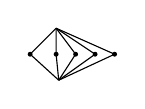
\begin{tikzpicture}[scale=.33,baseline=0pt]\coordinate (a) at (0,1);\coordinate (b) at (.1,-1);\foreach \x in {-1,0,.75,1.5,2.25}{\draw (a)--(\x,0)--(b);\fill (\x,0) circle(2.7pt);}\end{tikzpicture}}\\=\text{fausse 5-base}} & \mathrm{Ens}_5\times\mathrm{Ens}_2 & \substack{\text{cf plus haut}\\2^\circ} & 15 & \substack{1,1,5,\\5,5,10}\\ \hline
 & \text{triade }\deleted{\unsure{\text{triang}}}\inserted{\text{ordonnée}} & \substack{\inserted{\mathrm{Ens}_3\times\mathrm{Ens}_3\times\mathrm{Ens}_3}\\\deleted{\unsure{\mathfrak S_3\times\mathfrak S_3\times\mathfrak S_3}}} & \substack{\mathfrak S_3\times\mathfrak S_3\times\mathfrak S_3\\\text{ordre }6^3=2^3.3^3=216} & 2^4.3.5=240 & 9,9,9\\ \hline
 & \text{triades}\quad /\!/\!/ & \substack{\unsure{\text{puiss.}|\text{perm.}}\text{ d'ordre }3\\\text{d'un ens card. }3\simeq\\\text{ens de card. }9\text{ avec partition}} & \substack{\mathfrak S_3.(\mathfrak S_3\times\mathfrak S_3\times\mathfrak S_3)\\\text{card }6^4=2^4 3^4} & 2^3.5=40 & 27\\ \hline
 & \text{grilles 3-carrée}\unsure{\text{s}} & \substack{\text{comme dessus, avec}\\\text{une partie distinguée}} & \mathfrak S_2.(\mathfrak S_3\,\mathfrak S_3\,\mathfrak S_3) & 2^3.3.5=120 & 9,18\\ \hline
 & \substack{\text{arête}\quad\text{---}\\\simeq\text{triangle pointé}} &  &  &  & \\ \hline
 & \substack{\text{arcs}\quad\longrightarrow\\\sim\text{ triangle ordonné}} &  &  &  & \\ \hline
 & \text{triangles }\triangle &  &  &  & \\ \hline
 & \text{
\begin{tikzpicture}[baseline=0pt,scale=.35]\draw (-.6,.8)--(0,-.35)--(.6,.8);\foreach \x/\y in {-.6/.8,0/-.35,.6/.8}{\fill (\x,\y) circle(3pt);}\end{tikzpicture}} &  &  &  & \\ \hline
\unsure{\frac{120}{16}|13^\circ,\ 16} & \left(\text{
\begin{tikzpicture}[baseline=0pt,scale=.34]\draw (0,0)--(1.4,0);\fill (0,0) circle(3.4pt);\fill (1.4,0) circle(3.4pt);\fill (.7,.7) circle(2.8pt);\end{tikzpicture}}\right)\simeq(\text{arcs}) &  &  &  & 
\end{array}$}}
% archive sheet number: 61
